\chapter{LightNVM 寫入流程之修改設計}
\indent
本論文為提升 Garbage Collection 的效率,以及降低 Garbage Collection 的次數,而提出此設計。透過實作新的演算法,將其與 LightNVM 既有的寫入流程結合,如此一來,LightNVM 在寫入時,會透過這個方法挑選寫入位置,以達成提升效率的目的。

%本論文為增加RF Refactoring的功能,以及避免手動重構測試腳本及測試資源時,所造成的搜尋缺漏和取代錯誤,因而提出此設計。透過實作新的重構功能,將其與Eclipse中既有的外掛程式結合,團隊使用此工具選擇所需的重構方法進行重構時,其將利用Eclipse中的視圖(Views)及視窗(Dialogs)提供使用者做所需的選擇及輸入,進而完成重構的流程。

%\section{挑選新增之重構方法}\label{s3.1}
%\indent
%重構方法十分多種,劉冠志論文\cite{LIU-Thesis}是以國立台北科技大學軟體系統實驗室產學合作中,測試專案的測試團隊的重構需求為主,因此本論文也將以團隊的需求為主進行重構工具的擴充。
%
%\indent
%團隊開發測試腳本時,在過去所開發的測試腳本中發現含有自己所需的測試步驟,當下直接拿取做使用,且未立刻進行抽取成關鍵字的重構,導致重複步驟的產生,後續只能手動搜尋是否有重複步驟進而重構。此外,當團隊需要使用其他測試腳本已經撰寫好的關鍵字時,為了團隊的開發風格,時常需要將關鍵字宣告移動到其他測試資源中,因而必須手動檢查其餘使用到關鍵字的測試腳本是否正常,都十分地花費時間。根據上述,本論文將以抽取重複步驟成為新關鍵字、移動關鍵字宣告作為擴充之重構功能。
\section{初始化時修改為準備四個 Line}\label{s3.1}
\indent
在初始化時,LightNVM 會先準備好一個 Line,後續有檔案系統傳遞給 LightNVM 寫入要求時,就會從這個 Line 開始寫入,滿了之後會繼續挑選下一個有空間的 Line 來使用,因此我們為了將資料分開寫入,要修改為在初始化時先準備好四個 Line,以便之後的寫入分群使用。

\begin{figure}[H]
    \centering
    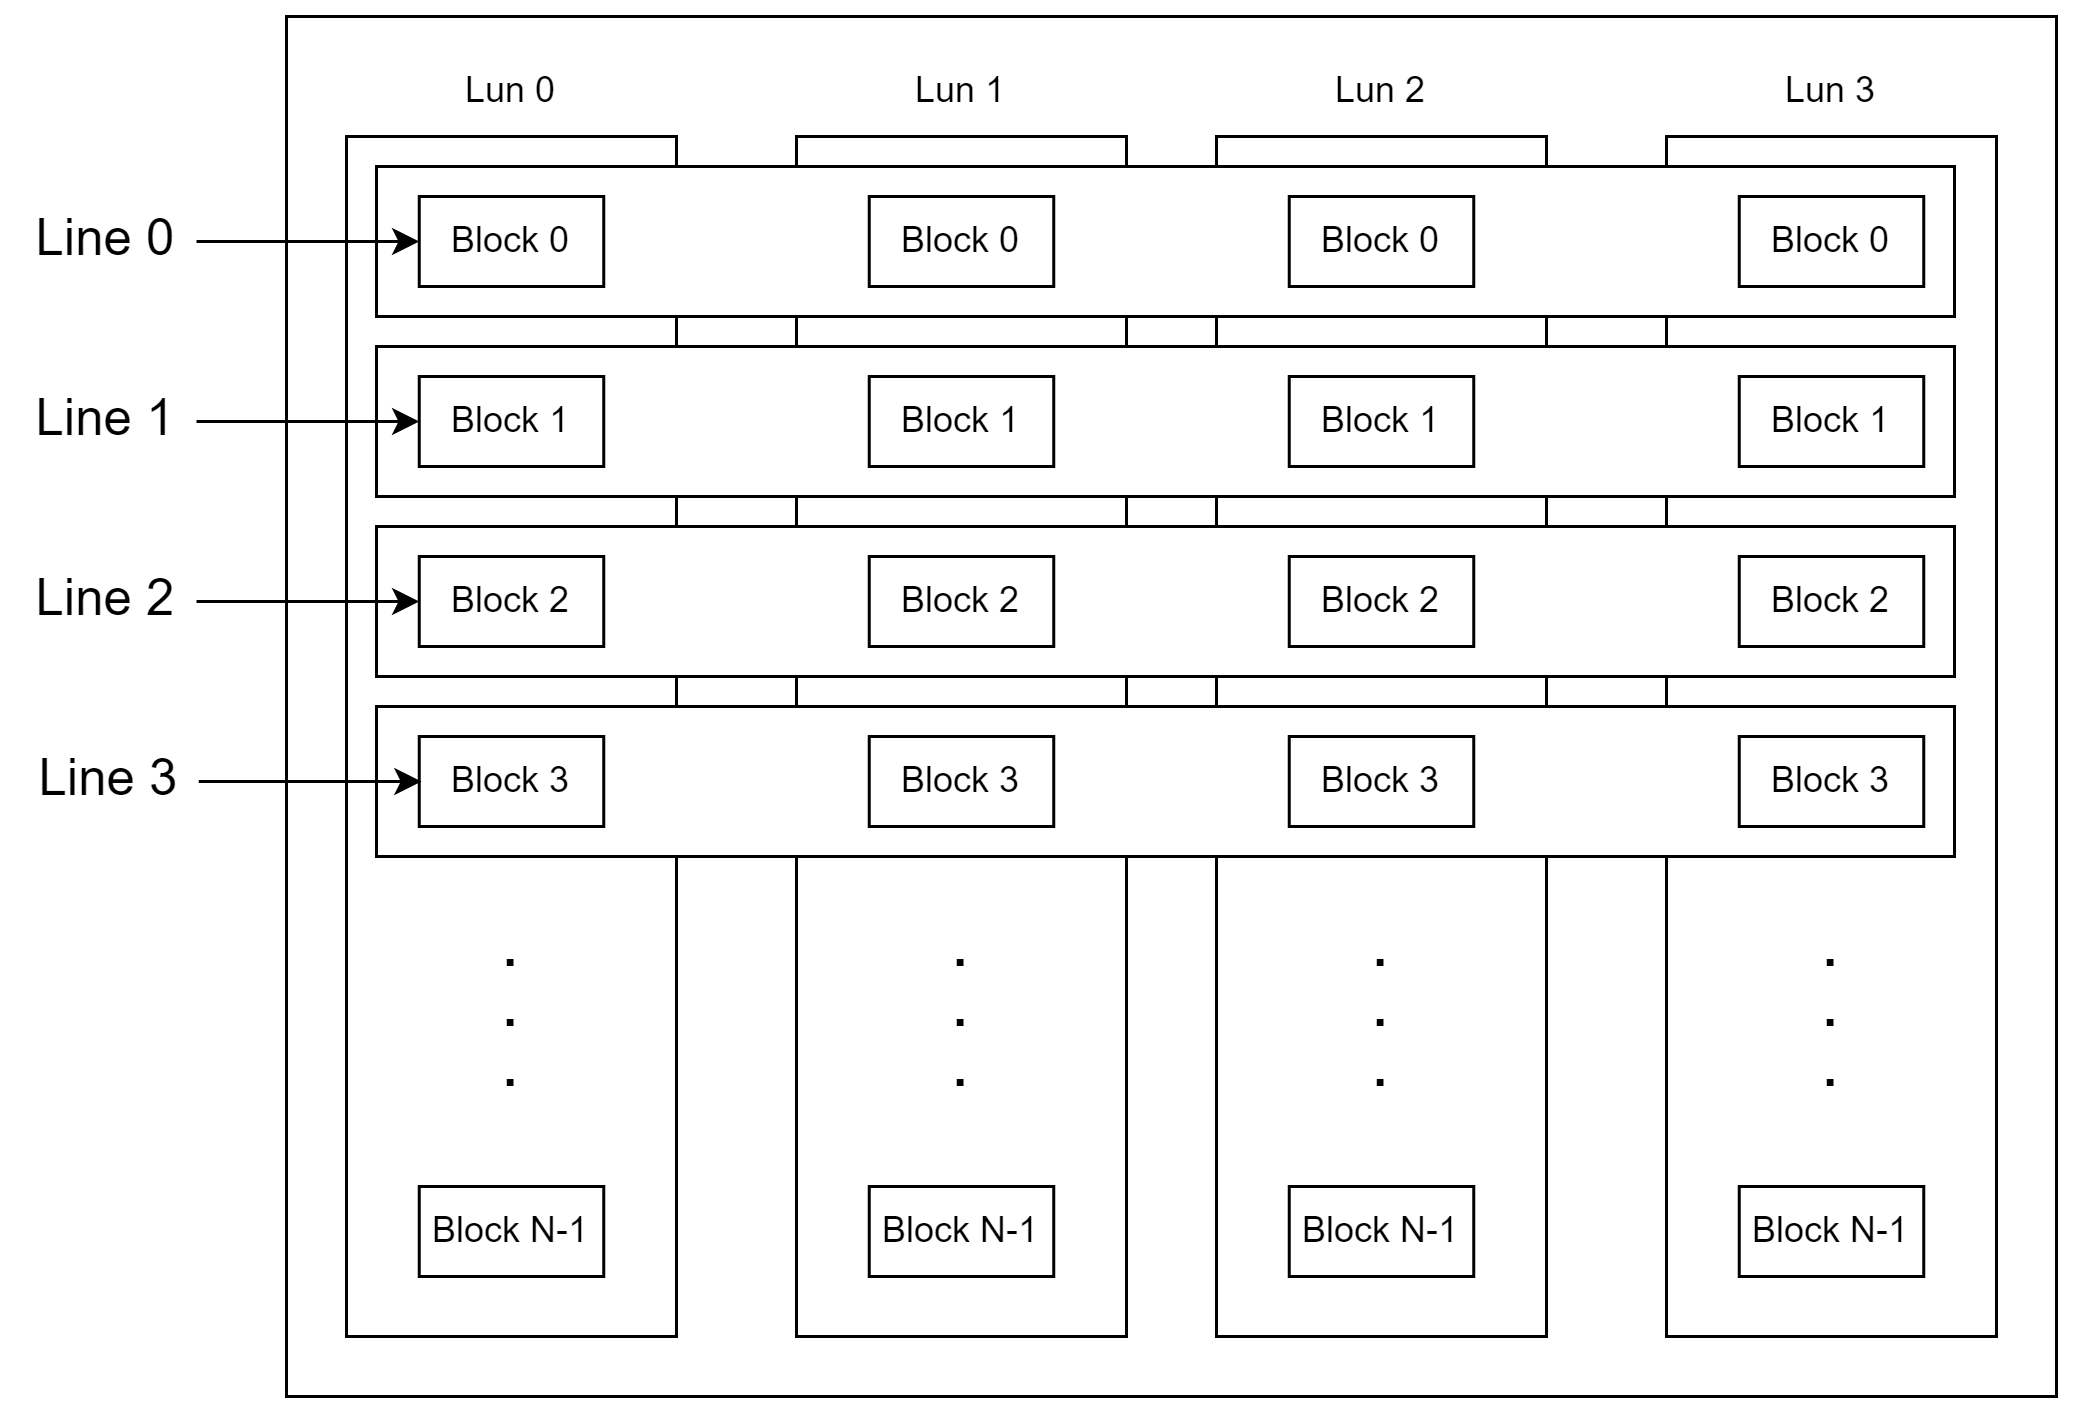
\includegraphics[width=0.8\textwidth]{picture/ch3/4Line.png}
    \caption{準備四個 Line 之示意圖}
    \label{f3.1}
\end{figure}

\section{處理檔案系統要求之流程}\label{s3.2}
\indent
檔案系統提出 Request 要求之後,LightNVM 會對 Request 拆解,儲存成 LightNVM 自己容易處理的形式,但是在拆解的同時,會損失一些資訊,所以首先我們要先在拆解 Request 之前把 Request 的大小先從 bio 擷取出來,用大小來判斷這個 Request 的資料屬於哪一個分群,並將資訊塞入 LightNVM 用來儲存 Request 的地方 - Ring Buffer 之中,最後再計算平均值,給下次 Request 傳進時使用。

\subsection{擷取 Request 大小並判斷分群}\label{s3.2.1}
\indent
在得到 Request 大小時,我們需要從檔案系統傳給 LightNVM 的資料結構 bio 之中,找到 Request 大小的值;由於我們需要前一萬筆 Request 大小的平均值,所以得到大小之後將其乘以 0.0001 倍再與我們加入 LightNVM 的平均值乘以 0.9999 倍之後相加

\subsection{擷取 Request 大小並計算平均值}\label{s3.2.3}
\indent
在得到 Request 大小時,我們需要從檔案系統傳給 LightNVM 的資料結構 bio 之中,找到 Request 大小的值;由於我們需要前一萬筆 Request 大小的平均值,所以得到大小之後將其乘以 0.0001 倍再與我們加入 LightNVM 的平均值乘以 0.9999 倍之後相加

\begin{figure}[H]
    \centering
    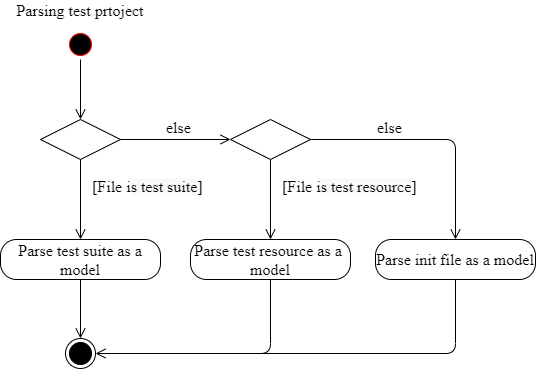
\includegraphics[width=0.7\textwidth]{picture/Parse_test_project.png}
    \caption{解析測試專案之活動圖}
    \label{f3.2}
\end{figure}

\subsection{創立新關鍵字}\label{s3.1.2}
\indent
透過\ref{s3.2.1}節所得到的AST模型,可從其中指定測試檔案中的步驟範圍,並且將其做為新關鍵字的測試步驟,以此創立新關鍵字。在決定所要抽取的測試步驟範圍時,必須為其檢查是否有使用未宣告在被抽取步驟的變數,一旦有此類型之變數,則需將其做為新關鍵字之參數,最後在指定的檔案中創立新關鍵字。圖\ref{f3.3}為創立新關鍵字的詳細活動。

\begin{figure}[H]
    \centering
    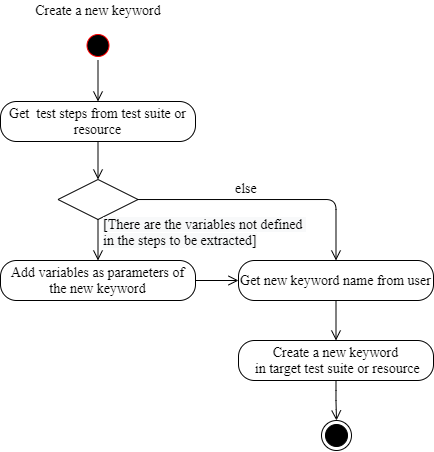
\includegraphics[width=0.55\textwidth]{picture/Create_a_new_keyword.png}
    \caption{創立新關鍵字之活動圖}
    \label{f3.3}
\end{figure}

\subsection{搜尋所有相關重複步驟並取代}\label{s3.2.3}
\indent
決定新關鍵字中的測試步驟時,將從\ref{s3.2.1}節取得的AST模型搜尋重複步驟,而是否為重複步驟將由三種條件定義,分別是與新關鍵字的測試步驟順序是否相同、使用的關鍵字是否命名相同、參數數量是否相同,由於測試開發人員在遇到能夠重複使用的測試步驟時,經常會將其拿取並直接使用於其他測試腳本中,並且當下沒有立刻進行抽取關鍵字之重構,因此才會制定上述條件來定義重複步驟,確保能夠搜尋到相對應資訊。首先確認檔案是否為測試套件,如是則檢查其測試案例內及關鍵字宣告內的測試步驟是否符合重複步驟之條件,皆符合才加入搜尋結果;反之則認定為測試資源,檢查其關鍵字宣告內的測試步驟是否符合上述條件,並且加入搜尋結果。此外,一旦發現符合條件的測試步驟位於不同的關鍵字或測試案例中時,需將其判別為非重複步驟,進而得出重複步驟的清單。

\indent
取得重複步驟清單後,必須提供選取需被取代的重複步驟之功能,藉此使用者可依照不同測試腳本的狀況進行挑選,使此重構能夠更加準確。圖\ref{f3.4}為搜尋重複步驟並取代的詳細活動。

\begin{figure}[H]
    \centering
    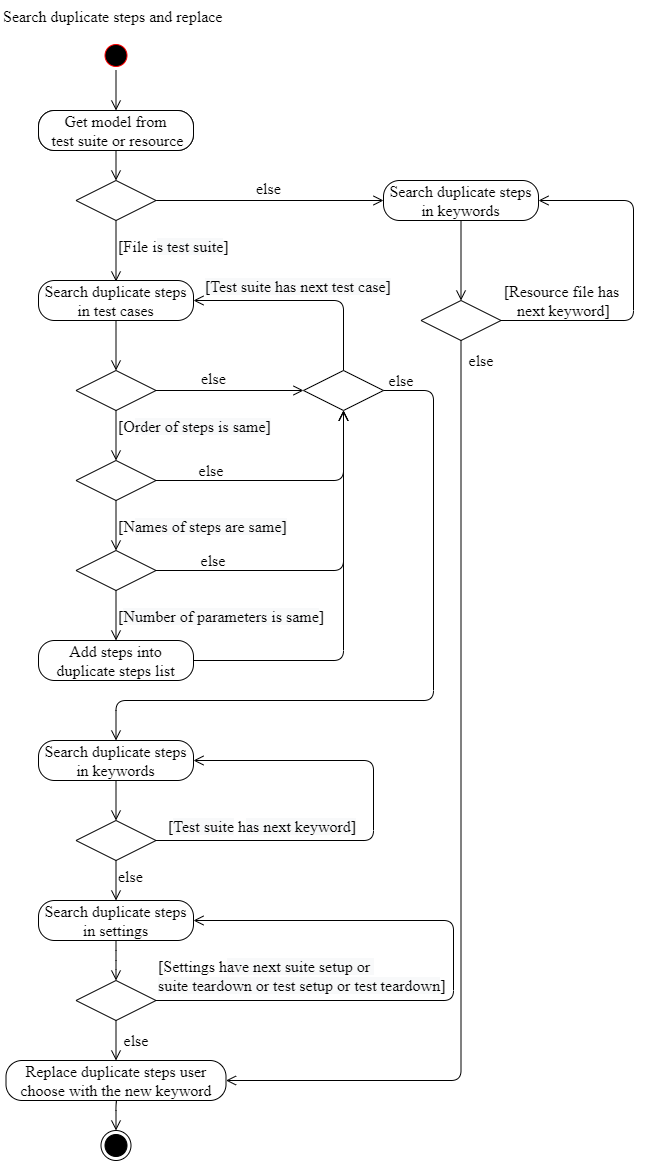
\includegraphics[width=0.7\textwidth]{picture/Search_duplicate_steps_and_replace.png}
    \caption{搜尋重複步驟並取代之活動圖}
    \label{f3.4}
\end{figure}

\subsection{搜尋未引入所需測試資源的測試檔案並自動引入}\label{s3.2.4}
%\indent
%在完成重複步驟的取代後,如果使用新關鍵字的測試腳本或測試資源未引入所需測試資源的話,將會導致測試腳本的錯誤,因此為了簡化進行重構後的檢查步驟,自動搜尋含有此錯誤的測試腳本或測試資源並自動修正是十分重要的。
\indent
在\ref{s3.2.3}節進行重複步驟的取代時,將會保留有使用新關鍵字的AST模型,透過留存的AST模型不必再次從專案全部檔案中進行搜尋,即可檢測是否都有確實引入新關鍵字所需的測試資源,能有效地提升重構效率。根據新關鍵字宣告所在檔案的位置及需要引入測試資源的檔案位置,便能為其引入所需測試資源的相對位置。圖\ref{f3.5}為搜尋未引入所需測試資源的測試檔案並自動引入的詳細活動。

\begin{figure}[H]
    \centering
    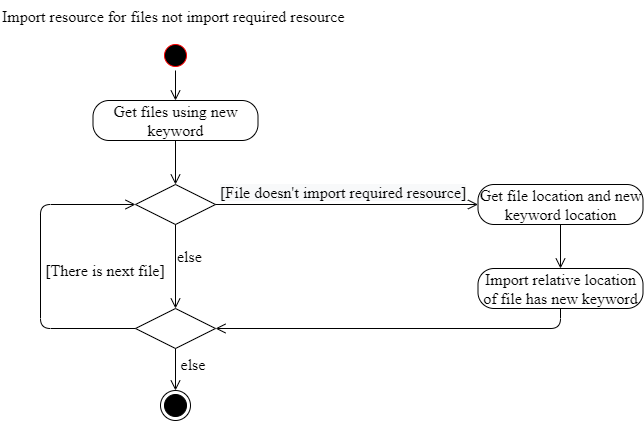
\includegraphics[width=0.7\textwidth]{picture/Import_resource_for_files_not_import_required_resource.png}
    \caption{搜尋未引入所需測試資源的測試檔案並自動引入之活動圖}
    \label{f3.5}
\end{figure}

\section{移動關鍵字宣告之流程}\label{s3.3}
\indent
在移動關鍵字宣告之前,必須與\ref{s3.2}節相同,提前解析測試專案下的所有測試檔案。移動關鍵字宣告至指定的測試資源後,必須檢查有使用被移動關鍵字的測試檔案,是否有引入所需之測試資源,最後進行引入之動作。圖\ref{f3.6}為移動關鍵字宣告之全部活動,以下將分別介紹各項活動。

\begin{figure}[H]
    \centering
    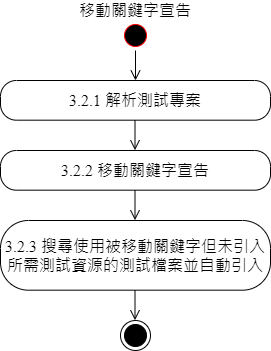
\includegraphics[width=0.4\textwidth]{picture/Move_definition_of_keyword.png}
    \caption{移動關鍵字宣告之活動圖}
    \label{f3.6}
\end{figure}

\subsection{解析測試專案}
\indent
此活動將與\ref{s3.2.1}節介紹相同,於移動關鍵字宣告之前解析測試專案中的測試檔案,並將其解析完成的AST模型儲存於記憶體,後續即可用來完成重構需求。

\subsection{移動關鍵字宣告}\label{s3.3.2}
\indent
在解析完測試專案後,指定所要移動的關鍵字宣告及新的測試資源位置,並將原先的關鍵字宣告進行移除,且將被移除的關鍵字宣告新增至新的測試資源中,以此完成關鍵字宣告之移動。圖\ref{f3.7}為移動關鍵字宣告的詳細活動。

\begin{figure}[H]
    \centering
    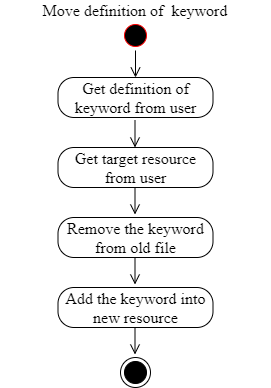
\includegraphics[width=0.4\textwidth]{picture/Move_definition_of_keyword_2.png}
    \caption{移動關鍵字宣告之活動圖}
    \label{f3.7}
\end{figure}

\subsection{搜尋使用被移動關鍵字但未引入所需測試資源的測試檔案並自動引入}\label{s3.3.3}
\indent
移動關鍵字宣告後,首先要搜尋有引入原先關鍵字宣告所在之檔案位置,且使用與關鍵字宣告同名關鍵字的測試檔案,藉此取得原先已使用被移動關鍵字的測試檔案,後續檢查其是否有引入被使用關鍵字所需的新測試資源,如果未引入所需測試資源則自動為其引入與新測試資源之相對路徑。圖\ref{f3.8}為搜尋使用被移動關鍵字但未引入所需測試資源的測試檔案並自動引入的詳細活動。

\begin{figure}[H]
    \centering
    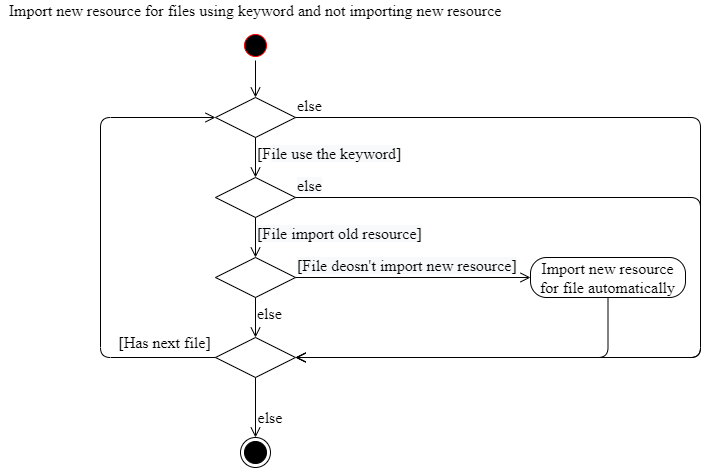
\includegraphics[width=1.0\textwidth]{picture/Import_resource_for_files_using_keyword_and_not_import_old_resource.png}
    \caption{搜尋使用被移動關鍵字但未引入所需測試資源的測試檔案並自動引入之活動圖}
    \label{f3.8}
\end{figure}

\section{將新重構功能結合至Eclipse既有之外掛程式}\label{s3.4}
\indent
RF Refactoring是Eclipse中的外掛程式,因此本論文將參考劉冠志論文\cite{LIU-Thesis}中所介紹之Eclipse外掛程式開發方法,將新重構功能結合至RF Refactoring中。

%\subsection{建立開發外掛程式之環境}
%\indent
%Plug-in Development Environment(PDE)\cite{PDE}是Eclipse中提供開發人員進行外掛程式開發的工具,其中提供了多種協助開發的功能,例如:創立專案、除錯、測試、建置專案、部屬等等。本論文將在PDE中引入既有外掛程式之專案,進行新重構功能之擴充。

%\subsection{利用Eclipse中延伸點與應用程式介面進行擴充}
%\indent
%\ref{s2.4}節中提及了Eclipse的擴充機制,而Eclipse中含有十分豐富的延伸點與各種應用程式介面,透過不同的延伸點與應用程式介面的結合,外掛程式可以更多元地使用Eclipse上的各種功能,例如:監聽使用者操作進而做出後續反應、取得工作區檔案中的各項資訊提供外掛程式使用等等。本論文透過此擴充機制能夠更加簡化使用者重構之動作,且更方便地新增重構功能。

%\subsection{增加command元素}\label{s3.4.3}
%\indent
%在Eclipse中command是一個行為的描述,但與實際行為操作並無相關,其行為操作是由handler所定義,而一個command可以擁有多個handler,但在一個時間點上只會將行為託付給一個handler。Eclipse提供了commands的延伸點,開發人員能夠藉此新增command以及定義其種類。本論文將為已有三個command的commands延伸點進行擴充,新增兩個command,分別為抽取重複步驟成為新關鍵字、移動關鍵字宣告,後續將新增handler為其定義實際行為。圖\ref{f3.9}為現有commands之延伸點。
%
%\begin{figure}[H]
%    \centering
%    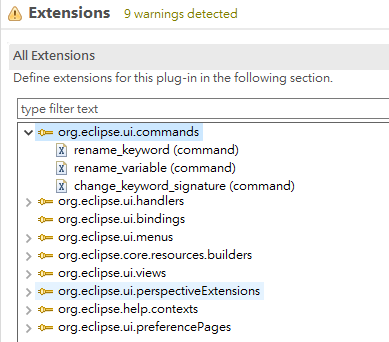
\includegraphics[width=0.8\textwidth]{picture/command_extension.PNG}
%    \caption{外掛程式現有之commands延伸點}
%    \label{f3.9}
%\end{figure}
%
%\subsection{透過handler定義新command的行為}
%\indent
%Eclipse提供了handlers的延伸點,讓開發人員能夠進行handler與command的連接,並且設定handler在不同條件下為啟用、禁用或非活動的狀態,如果handler處於禁用狀態,儘管收到了command的委託,也不會執行,而處於非活動的狀態時,command將不會被委託至此handler,因此在啟用狀態下,command將會委託此handler執行行為。本論文將為已有三個handler的handlers延伸點新增兩個handler,並將其與\ref{s3.4.3}節中的command進行連接,完成相對應的重構行為。圖\ref{f3.10}為現有handlers之延伸點。
%
%\begin{figure}[H]
%    \centering
%    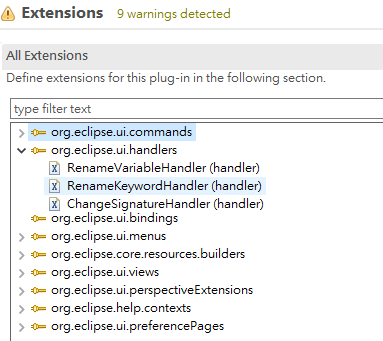
\includegraphics[width=0.8\textwidth]{picture/handler_extension.PNG}
%    \caption{外掛程式現有之handlers延伸點}
%    \label{f3.10}
%\end{figure}
%
%\subsection{將新command與選單介面結合}
%\indent
%Eclipse提供了menus的延伸點,讓開發人員能夠將客製化的選單新增至Eclipse框架上,提供使用者能夠操作其所需之功能,其中提供了以下幾種選單種類:
%
%\begin{itemize}
%
%\item\textbf{主選單(Main menu)}
%
%\item\textbf{主工具列(Main toolbars)}
%
%\item\textbf{修剪選單(Trim)}
%
%\item\textbf{視圖選單/工具列(View menus/Toolbars)}
%
%\end{itemize}
%
%\indent
%此外選單介面可與不同元件結合,例如:control、command、menu等等,讓客製化選單能夠更加多元。本論文將於現有menus延伸點的客製化選單中,結合\ref{s3.4.3}節中所新增之command,讓使用者能夠依照其需求選擇選單中的功能,並將command委託至handler執行。圖\ref{f3.11}為現有menus之延伸點。
%
%\begin{figure}[H]
%    \centering
%    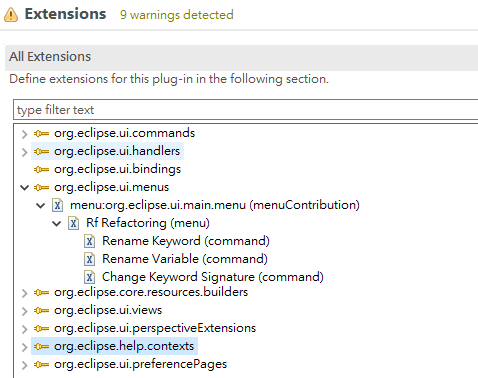
\includegraphics[width=0.8\textwidth]{picture/menu_extension.PNG}
%    \caption{外掛程式現有之menus延伸點}
%    \label{f3.11}
%\end{figure}

%\subsection{透過視圖及視窗協助重構功能執行}
%\indent
%Eclipse提供了views延伸點,開發人員可藉此新增客製化的視圖(View),而視圖為工作區內的可視化元件,其可被用來顯示command執行結果資訊或新增額外的使用者元件等等,圖\ref{f3.12}為現有外掛程式的客製化視圖,其提供使用者選擇所要重新命名的參考。本論文將於現有views延伸點新增兩個不同的客製化視圖,分別提供使用者選擇重複步驟或目標檔案,以此協助重構功能之執行。
%
%\begin{figure}[H]
%    \centering
%    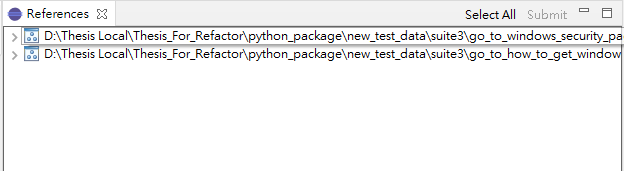
\includegraphics[width=1.0\textwidth]{picture/choose_keyword_view.PNG}
%    \caption{現有外掛程式的客製化視圖}
%    \label{f3.12}
%\end{figure}
%
%\indent
%視窗(Dialog)是SWT(Standard Widget Toolkit)\cite{SWT}中所提供的視窗元件,其可透過開發人員自行設計介面,以達到所需之功能,圖\ref{f3.13}為現有外掛程式的客製化視窗,其提供使用者輸入重新命名的關鍵字名稱。本論文將新增兩個視窗介面,提供使用者創建新關鍵字及用新關鍵字取代重複步驟之功能使用,協助整體重構功能之執行。
%
%\begin{figure}[H]
%    \centering
%    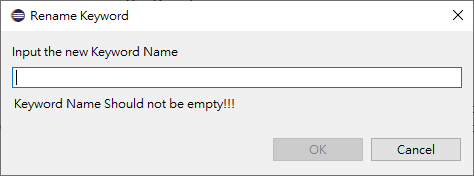
\includegraphics[width=0.7\textwidth]{picture/Rename_keyword_dialog.PNG}
%    \caption{現有外掛程式的客製化視窗}
%    \label{f3.13}
%\end{figure}